\documentclass[preprint]{sig-alternate-sigmod08}
\usepackage{url}
\usepackage{stmaryrd}
\usepackage{epsfig}
\usepackage{alltt}
\usepackage{times}
\usepackage{code}
\usepackage{xspace}

% \pdfpagewidth=8.5in
% \pdfpageheight=11in

\renewcommand{\floatpagefraction}{0.9}
\renewcommand{\dbltopfraction}{0.9}
\renewcommand{\dblfloatpagefraction}{0.9}
\addtolength{\textfloatsep}{-8pt}
\addtolength{\dbltextfloatsep}{-8pt}

\newcommand{\cut}[1]{}

\newcommand{\appref}[1]{Appendix~\ref{#1}}
\newcommand{\secref}[1]{Section~\ref{#1}}
\newcommand{\tblref}[1]{Table~\ref{#1}}
\newcommand{\figref}[1]{Figure~\ref{#1}}
\newcommand{\listingref}[1]{Listing~\ref{#1}}
%\newcommand{\pref}[1]{{page~\pageref{#1}}}

\newcommand{\eg}{{\em e.g.}}
\newcommand{\cf}{{\em cf.}}
\newcommand{\ie}{{\em i.e.}}
\newcommand{\etc}{{\em etc.\/}}
\newcommand{\naive}{na\"{\i}ve}
\newcommand{\role}{r\^{o}le}
\newcommand{\forte}{{fort\'{e}\/}}
\newcommand{\appr}{\~{}}

\newcommand{\bftt}[1]{{\ttfamily\bfseries{}#1}}
\newcommand{\kw}[1]{\bftt {#1}}
\newcommand{\Pthen}{\kw{Pthen}}
\newcommand{\pads}{\textsc{pads}}
\newcommand{\padsl}{\textsc{padsl}}
\newcommand{\padst}{\textsc{pads/t}}
\newcommand{\datatype}{\textsc{PADS/T}}
%\newcommand{\datatype}{\textsc{DataType}}
\newcommand{\C}{\textsc{C}}
\newcommand{\perl}{\textsc{Perl}}
\newcommand{\ml}{\textsc{ml}}
\newcommand{\sml}{\textsc{sml}}
\newcommand{\smlnj}{\textsc{sml/nj}}
\newcommand{\java}{\textsc{java}}
\newcommand{\ddl}{\textsc{ddl}}
\newcommand{\xml}{\textsc{xml}}
\newcommand{\datascript}{\textsc{DataScript}}
\newcommand{\packettypes}{\textsc{PacketTypes}}
\newcommand{\erlang}{\textsc{Erlang}}

\newcommand{\Core}{Ad hoc}
\newcommand{\core}{ad hoc}
\newcommand{\pvalue}{\core{} value}
\newcommand{\ppat}{\core{} pattern}
\newcommand{\ptype}{\core{} type}

\newcommand{\padsc}{\textsc{pads}/\C{}}
\newcommand{\padsml}{\textsc{pads}/\ml{}}

\newcommand{\dibbler}{Sirius}
\newcommand{\ningaui}{Altair}
\newcommand{\darkstar}{Regulus}

\newcommand{\pdgood}{{\tt G}}
\newcommand{\pdbad}{{\tt B}}
\newcommand{\pdnest}{{\tt N}}
\newcommand{\pdsem}{{\tt S}}
\newcommand{\ptypes}{T}
\newcommand{\patreadpd}[2]{{\tt #1<<#2>>}}
\newcommand{\btm}{\cd{BOT}}


\newcommand{\lsem}{{[\![}}
\newcommand{\rsem}{{]\!]}}


\newcommand{\figHeight}[4]{\begin{figure}[tb]
	\centerline{
	            \epsfig{file=#1,height=#4}}
	\caption{#2}
	\label{#3}
	\end{figure}}

%% Environment for typesetting BNF grammars. Uses display math mode.
\newenvironment{bnf}
     {%% local command definitions:
        %% BNF definition symbol
      \def\->{\rightarrow}
%%      \def\::={{::=} &}
      \def\::={\bnfdef &}
      \def\|{\bnfalt}
      \newcommand{\name}[1]{\text{##1}}
        %% non-terminal
      \newcommand{\nont}[1]{{##1}}
      \newcommand{\meta}[1]{& ##1 &}
      \newcommand{\descr}[1]{& \text{// ##1}}
      \newcommand{\opt}[1]{ [##1] }
      \newcommand{\opnon}[1]{\opt{\nont{##1}}}
      \newcommand{\none}{\epsilon}
      \newcommand{\nwln}{\\ &&&}
      \newcommand{\nlalt}{\\ && \| &}
      \[\begin{array}{lrlll}
     }
     {\end{array}\]}

\newcommand{\mcd}[1]{\mathtt{#1}}
\newcommand{\ppair}[3]{#1{:}#2 \mathrel{**} #3}
\newcommand{\parray}[3]{#1\;\mcd{Parray}(#2,#3)}
\newcommand{\pset}[3]{\{#1{:}#2\,|\,#3\}}
\newcommand{\pstream}[1]{#1\;\mcd{stream}}
\newcommand{\precord}[1]{\{\{#1\}\}}

\newcommand{\mono}[1]{\texttt{#1}}
\newcommand{\dibbler}{Sirius}
\newcommand{\ningaui}{Altair}
\newcommand{\darkstar}{Regulus}

\newcommand{\abstractdm}{abstract data model}
\newcommand{\concretedm}{concrete data model}
\newcommand{\typeddm}{type-specialized concrete data model}
\toappear{}
\title{LearnPADS: Automatic Tool Generation from Ad Hoc Data}

\numberofauthors{3} 
\author{\alignauthor Kathleen Fisher \\
\affaddr{AT\&T Labs Research}
\email{kfisher@research.att.com}
\alignauthor David Walker \\
\affaddr{Princeton University}\\
\email{dpw@cs.princeton.edu}
\alignauthor Kenny Zhu \\
\affaddr{Princeton University}\\
\email{kzhu@cs.princeton.edu}
%\affaddr{Galois Connections}\\
%\email{peter@galois.com}}
}
%\eat{
%\additionalauthors{Robert Gruber (Google, 
%  {\texttt{gruber@google.com}}), while at AT\&T Labs and Xuan Zheng (Univ. of Michigan, 
%  {\texttt{xuanzh@eecs.umich.edu}}), supported by 
%	 AT\&T Labs and NSF DMS 0354600.}}
%
%\date{\today}

\begin{document}

\maketitle
\begin{abstract}
In this demonstration, we will present \learnpads, 
a fully automatic system for generating
ad hoc data processing tools.  When presented with a collection of
ad hoc data, the system (1) analyzes the data, (2) infers a 
\pads{}~\cite{fisher+:pads,fisher+:popl06} description, (3) 
generates parser, printer, validation and traversal libraries and (4)
links these libraries with format-independent  
tool suites to form stand-alone applications.  These applications provide
statistical analysis, \xml{}
conversion, CSV conversion, the ability to query with the 
Galax XQuery engine~\cite{fernandez+:padx}, and the ability to 
graph selected data elements, all
directly from ASCII ad hoc data without human intervention.
SIGMOD attendees will see both the user experience with \learnpads{} and
the internals of the multi-phase inference algorithm which lies at
the heart of the system. 
\end{abstract}

\section{Introduction}
An {\em ad hoc data source} is any semistructured data source
for which useful data analysis and transformation tools
are not widely available. XML, HTML and CSV are {\em not} 
ad hoc data sources as there are numerous programming libraries,
query languages, manuals and other resources dedicated to
helping analysts manipulate data in these formats.
Despite the existence of these standard formats, ad hoc data arises
often in many fields ranging from computational biology to finance to networking.

The goal of the \pads{} project~\cite{padsweb} is to improve the
productivity of data analysts who must regularly cope with new and evolving
ad hoc data sources.  Our core technology is a
domain-specific language in which programmers can specify the
structure and expected properties of ad hoc data sources, whether they
be ASCII, binary, Cobol or a mixture of formats~\cite{fisher+:pads,fisher+:popl06}.  These
specifications, which resemble extended type declarations from
conventional programming languages, are compiled into a suite of
programming libraries, such as parsers and printers, and 
end-to-end data processing tools including a query engine 
and several format translators~\cite{fernandez+:padl,fernandez+:padx,mandelbaum+:pads-ml}.

Unfortunately, it often takes substantial time and expertise to write
a \pads{} description for a new ad hoc data source -- days or even
weeks for complex sources.  To address this problem, we have developed
a multi-phase algorithm that automatically infers the structure of
ASCII data sources and produces \pads{} descriptions.  From these
descriptions, \learnpads{} generates libraries and the set of tools
supported by the \pads{} system.  Analysts can simply use these tools
or write their own programs to process the data using the generated
parser and printer.  The technical details of the inference system 
appear in our recent paper
%at the ACM SIGPLAN Conference on Principles of Programming Languages
\cite{fisher+:dirttoshovels}.  The web page
\url{http://www.padsproj.org/learning-demo.html} has a live
demo, which would constitute a portion of our demonstration
% at SIGMOD.

Space precludes a discussion of related work here; however, our recent
paper~\cite{fisher+:dirttoshovels} contains an overview of related
work in information extraction, regular expression inference, and
schema induction.  

\section{User Experience}

Individual network administrators, systems researchers and large 
corporations like AT\&T must constantly monitor the performance,
reliability and security of their systems.
In the process, they often have to ingest new kinds of data
as new kinds of machines with new log file formats come
online.  This ingestion process requires understanding the physical
layout of the data source and properties of the data such as value
ranges and correlations.  In this paper, we use a tiny
web server log file {\tt ai.3000} as a simple example of the kinds of
data sources such analysts must develop tools for. A sample record has
the form:

{\small
\begin{verbatim}
www.proxy.aol.com - - [16/Oct/1997:08:20:45 -0700] 
  "GET /tk/pan.gif HTTP/1.0" 200 15944
\end{verbatim}
}

\noindent
To process this data with our system, the user would enter


{\small
\begin{verbatim}
kzhu@myhost> learn data/ai.3000 
\end{verbatim}
}

\noindent
This command analyzes the web server data and generates a collection
of useful artifacts including each of the following.

\begin{itemize}
\item A complete {\em \pads{} description} that analysts can
examine for syntactic information about their data source.  This description 
can be edited, if desired, and used to regenerate any of the 
tools listed below or to generate a collection of C language libraries for 
parsing, printing, \etc
\item An {\em accumulator} tool
that produces a statistical report about the data source.  This
tool may be run on any data sharing the format of
the original data.  It catalogs the number of errors
and the distribution of values in all fields of the data.
Figure \ref{fig-accum-report} shows the result of applying this
program to {\tt ai.3000}.
\item A {\em formatting} program that converts
the ad hoc data into a tabular form with user-defined delimiters
such as commas or vertical bars for loading the data into a relational database.
\item An {\em \xml{} translator} to convert
raw data in the original format into a canonical \xml{} representation.  
%Figure \ref{fig-xml} presents a fragment of
%the \xml{} that results from the conversion process.
\item A graphing tool that allows analysts to extract and plot fields
of the raw data using GNUPlot. Figure \ref{fig-graph} presents a graph of web
transaction volume during some time periods in a day, computed from
the {\tt ai.3000} data.
\end{itemize}
In the demo, we will run the format inferencing engine on a variety of
data formats.  We will show the resulting PADS descriptions and the
output of these generated programs when run on data similar to the
training data.

\begin{figure*}
\begin{center}
{\small
\begin{verbatim}
*****************************************************************************************************
<top> : struct Struct_149
*****************************************************************************************************
good vals:        3000   bad vals:          0    pcnt-bad:    0.000

[Describing each field of <top>]
... OMMITTED ...
+++++++++++++++++++++++++++++++++++++++++++++++++++++++++++++++++++++++++++++++++++++++++++++++++++++
<top>.var_70 : enum Enum_70
+++++++++++++++++++++++++++++++++++++++++++++++++++++++++++++++++++++++++++++++++++++++++++++++++++++
good vals:       3000    bad vals:          0    pcnt-bad:    0.000
  Characterizing enum Enum_70 values:  min POST (    0)  max GET (    1)
    => distribution of top 2 values out of 2 distinct values:
        val: GET (    1)    count:       2999  pcnt-of-good-vals:   99.967
        val: POST (    0)   count:          1  pcnt-of-good-vals:    0.033
. .  . . . . . . . . . . . . . . . . . . . . . . . . . . . . . . . . . . .
        SUMMING             count:       3000  pcnt-of-good-vals:  100.000
\end{verbatim}
}
\caption{A Fragment of the Accumulator Report}\label{fig-accum-report}
\end{center}
\end{figure*}

\begin{figure}[th]
\begin{center}
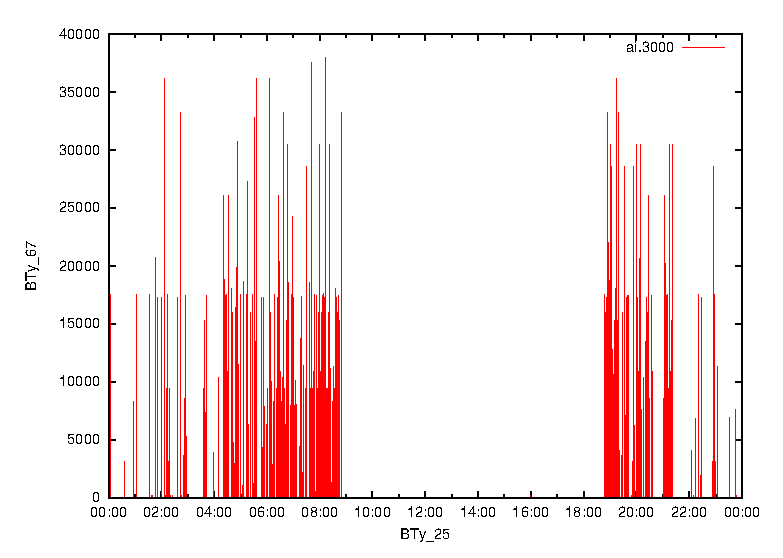
\epsfig{file=ai.3000.eps, width=0.9\columnwidth} 
\caption{A graph generated from ai.3000} \label{fig-graph}
\vspace*{-5mm}
\end{center}
\end{figure}

\section{How it works}
\begin{figure}
\begin{center}
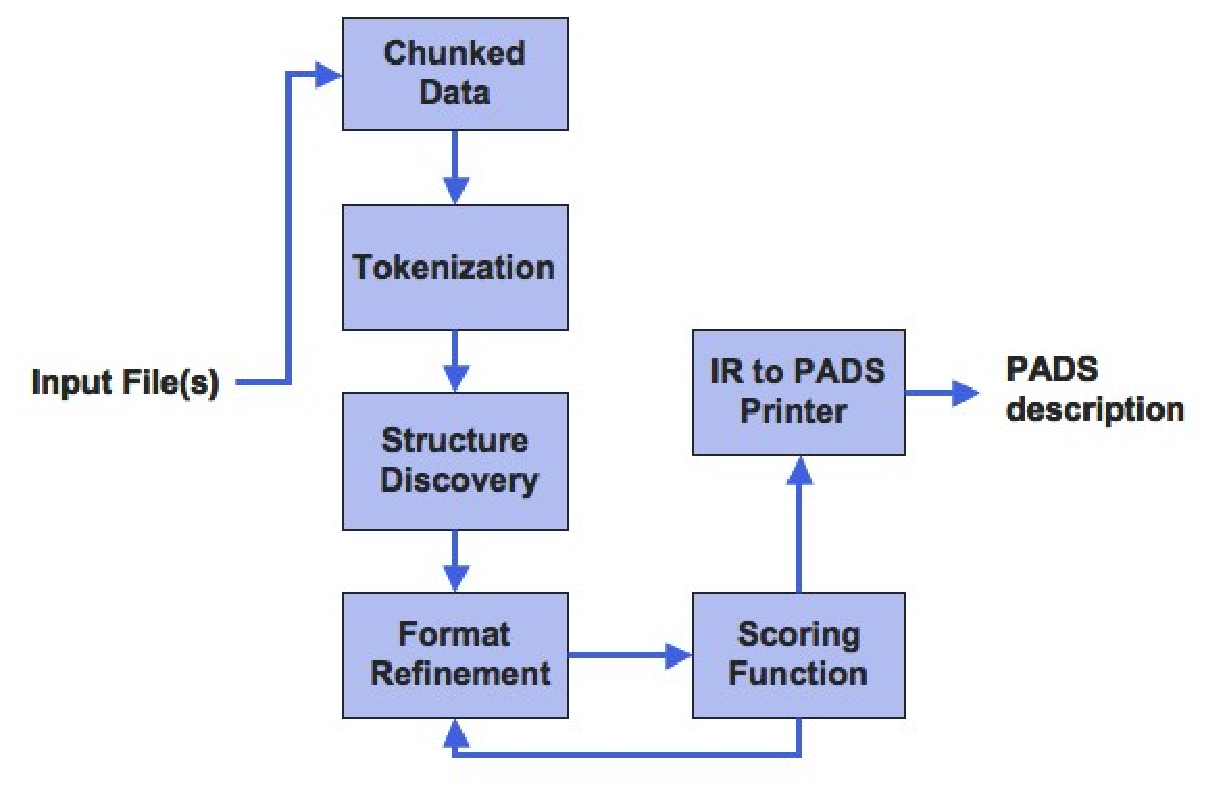
\epsfig{file=archi.eps, width=0.9\columnwidth}
\caption{Architecture of LearnPADS}
\vspace*{-5mm}
\label{fig-archi}
\end{center}
\end{figure}
After showing the experience of using our tool, we will demonstrate
how it works by walking through the steps of the algorithm on the
following simple data file:

{\small 
\begin{verbatim}
:123, 14:
:721, Harry:
:574, Hermione:
:9378, 56:
:12, Hogwarts:
:112, Ron:
\end{verbatim}
}

\figref{fig-archi} gives an overview of the architecture of the system.
The input data, or ``training set,'' is first partitioned into chunks;
each chunk is a piece of recurrent data such as a line, 
a paragraph, or a file (if the input consists of multiple files).
The user specifies this unit of repetition when invoking the tool.
Each chunk is then divided into a series of tokens.  Each
token can be a punctuation symbol, a number, a date, a time, or a number of other
basic types.  Our learning system has a tokenization scheme
skewed toward systems data, but users may specify a different scheme 
for their own domain through a configuration file.  For example,
computational biologists may want to specify new base types for DNA strings
or gene names.  When applied to our sample file,
this phase produces the following output, in which each line is a chunk
and each sequence within brackets is a token:

{\small
\begin{verbatim}
[:] [Int] [,] [White] [Int]    [:]
[:] [Int] [,] [White] [String] [:]
[:] [Int] [,] [White] [String] [:]
[:] [Int] [,] [White] [Int]    [:]
[:] [Int] [,] [White] [String] [:]
[:] [Int] [,] [White] [String] [:]
\end{verbatim}
}

\begin {figure*}[tbh]
\begin{center}
\begin{minipage}[t]{0.5\columnwidth}
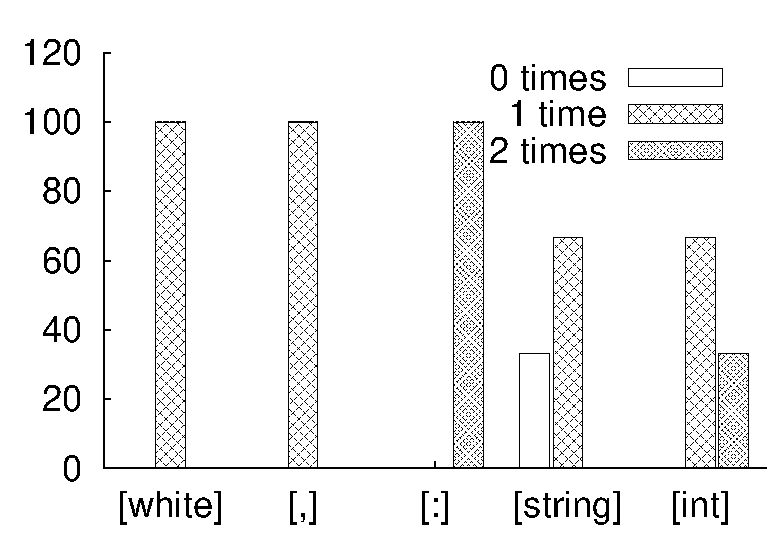
\epsfig{file=histogram0.eps, width=\columnwidth}
\end{minipage}
\hfill
\begin{minipage}[t]{0.5\columnwidth}
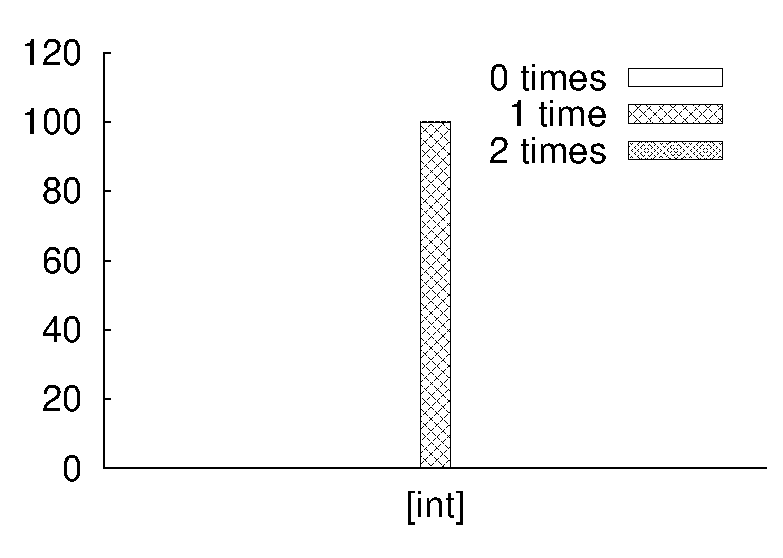
\epsfig{file=histogram1-1.eps, width=\columnwidth}
\end{minipage}
\hfill
\begin{minipage}[t]{0.5\columnwidth}
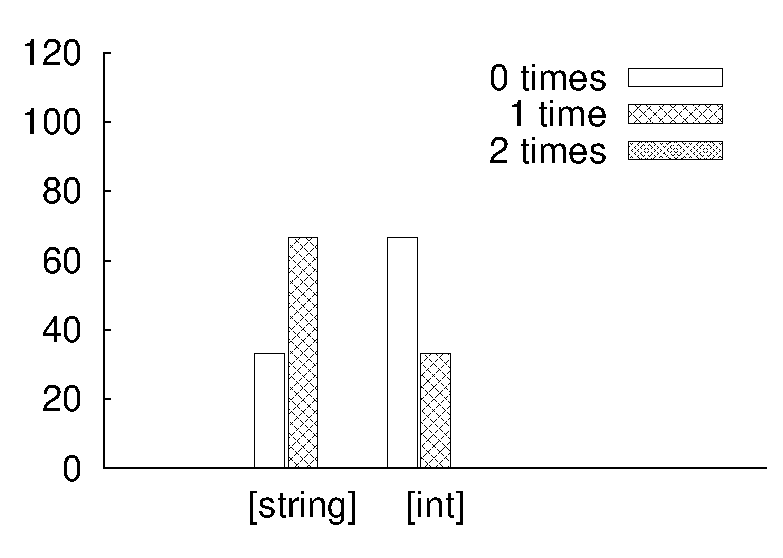
\epsfig{file=histogram1-2.eps, width=\columnwidth}
\end{minipage}
\caption{Histograms calculuated from sample data file (from left to right): 
(a) first iteration, (b) second iteration (context 1) 
and (c) second iteration (context 2)} \label{fig-hist}
\vspace*{-5mm}
\end{center}
\end{figure*}

In the structure discovery phase, we use a top-down, divide-and-conquer
scheme inspired in part by the work of Arasu and Garcia-Molina on
information extraction from web pages~\cite{arasu+:sigmod03}. 
This scheme calculates frequency distributions for tokens within
chunks.  It uses this information to
decide the top-level structure for the chunks, either a 
\tkw{Pstruct}, a \tkw{Parray}, or a \tkw{Punion}, corresponding to a
tuple, a variable-length sequence, or an alternation in the data.
The system then partitions the data accordingly
and the algorithm recursively analyzes subchunks. 

For example, when applied to our sample data file, the first iteration of this
process determines that the tokens
[White], [:], and [,] have similar frequency distributions
(histograms with 100\% coverage in one single spike) as shown in \figref{fig-hist}(a).
Hence we group these tokens
into a cluster and identify them as a \tkw{Pstruct}. 
The system then partitions the initial chunks into:

{\small
\begin{verbatim}
[:] <context 1> [,] [White] <context 2> [:]
\end{verbatim}
}
\noindent where \verb#[:]#, \verb#[,] [White]# and \verb#[:]# delimit
the subchunks.

In the second iteration, we compute histograms of the tokens in context 1 and
context 2, shown in \figref{fig-hist}(b) and \figref{fig-hist}(c) 
respectively. We can infer context 1 is a simple integer
as the token [Int] has 100\% coverage. In context 2,
the histograms for [String] and [Int] do not
show strong struct characteristics, so the algorithm introduces
a \tkw{Punion}.  

We represent the structure inferred by this recursive process
in an intermediate representation (IR) that has 
expressive power similar to the \pads{} language~\cite{fisher+:popl06}.  
We annotate each node in this representation with metadata
comprising a unique id, the coverage of the node,
and an information-theoretic score labelled ``raw'' that characterizes
how well that part of the description characterizes the data.  
The IR computed for our example file follows.

{\small
\begin{verbatim}
Pstruct(Id = BTy_20 6, raw: 432.183b)
  [Other](:) (Id = BTy_1 6, raw: 50.372b);
  Pstruct(Id = BTy_5 6, raw: 70.883b)
    [Pint] (Id = BTy_3 6, raw: 65.839b);
  End Pstruct;
  [Other](,) (Id = BTy_6 6, raw: 50.372b);
  [White] (Id = BTy_8 6, raw: 17.044b);
  Punion(Id = BTy_13 6, raw: 185.510b)
    Pstruct(Id = BTy_12 4, raw: 154.089b)
      [String] (Id = BTy_10 4, raw: 149.044b);
    End Pstruct;
    Pstruct(Id = BTy_17 2, raw: 24.377b)
      [Pint] (Id = BTy_15 2, raw: 19.332b);
    End Pstruct;
  End Punion;
  [Other](:) (Id = BTy_18 6, raw: 50.372b);
End Pstruct
\end{verbatim}
}

The format refinement phase analyzes the IR produced by structure discovery
and repeatedly applies value-independent and value-dependent
rewriting rules. 
The value-independent rules examine the inferred description 
to merge or otherwise rearrange components to improve the description.
Value-dependent rules introduce constants and enumerations by
analyzing the inferred description and the underlying
training data looking for fields with little or no 
variation. The value-dependent rules also infer
inter-field dependency information.
At any point in the refinement process,
many rewriting rules may apply; our algorithm chooses the rule
that optimizes an information-theoretic
scoring function based on the minimum description length
principle. The process stops when no further refinements are possible.
The result of this process on our running example is the following
refined IR:

{\small
\begin{verbatim}
Pstruct(Id = BTy_20 6, raw: 287.759b)
  [StringConst] ":" (Id = BTy_1 6, raw: 11.044b);
  [Pint] (Id = BTy_3 6, raw: 65.839b);
  [StringConst] ", " (Id = BTy_6 6, raw: 17.044b);
  Punion(Id = BTy_13 6, raw: 175.421b)
    [Pint] (Id = BTy_15 2, raw: 19.332b);
    [String] (Id = BTy_10 4, raw: 149.044b);
  End Punion;
 [StringConst] ":" (Id = BTy_18 6, raw: 11.044b);
End Pstruct
\end{verbatim}
}

Finally, a pretty printer translates the final IR into a legal PADS 
specification,  which the PADS compiler uses to generate
a suite of useful tools (Only the XML converter and the accumulator are included
in Fig. \ref{fig-archi}).  The PADS description inferred for our
sample data source follows:

{\small
\begin{verbatim}
Punion Union_13 {
       Pint64 var_15;
       PPstring var_10;
};
Precord Pstruct Struct_20 {
        ':';
        Pint64 var_3;
        ", ";
        Union_13 var_13;
        ':';
};
Psource Parray entries_t {
        Struct_20[];
};
\end{verbatim}
}

\eat{
\section{Conclusions}
The primary conclusion of our preliminary study 
is that it is possible to infer useful \pads{} descriptions 
from a sufficiently large corpus of training data.  Indeed,
with just a push of a button, we can now automatically generate
tools that convert raw data into XML and generate statistical reports.
Where it once took days or weeks to access and transform ad hoc data, it now
takes seconds.
and (2) generate a useful statistical report.  However, 
there is still much work to be done as the generated formats
often tend to overspecialize and turn out to be more complex than
their human-generated counterparts.
}



\bibliographystyle{abbrv}
\bibliography{pads}

\end{document}

